\chapter{Motorstyring på x- og y-akser samt sensor detektering}
\section{Indledning}
Dette afsnit har til formål at beskrive den unipolære styring af stepper motorerne der bevæger x- og y-akserne, og dermed, de to sensorer der skal detektere om der står en vinflaske i WinePrep.

Det er 2 stepper motorer af typen 28BYJ-48 der er valgt til at styre de to akser. For specifikationer af motoren henvises til databladet for 28BYJ-48 som kan findes i bilag xx.

Motoren er i forvejen kendt fra øvelsen om motorstyring i kurset Grænseflader til den fysiske verden (GFV), og det er på denne baggrund at de er valgt.

Den unipolære motorstyring er valgt frem for bipolær styring ud fra en overvejelse om moment og kompleksitet. For at være på den sikre side ift. at motoren har det nødvendige moment tændes to faser ad gangen i full step-mode.

De to sensorer er af typen GP2Y0A21YK, og er alene valgt ud fra Embedded Stocks udvalg. Sensorer med en rækkevidde fra 0 cm havde været foretrukket da designet af WinePreps ramme ville have været nemmere at implementere sensorerne i. Datablad for sensorerne kan findes i bilag xx.

\section{Design og implementering}
Motorernes spoler styres, via et ULN2003AN board, fra en PSoC 5LP. Sensorerne aflæses direkte på PSoCen.

\subsection{PSoC}
Nedenfor beskrives PSoC håndteringen af motorer og sensorer, hvilke interne PSoC komponenter der har været nødvendige for dette samt pin konfigurering og kode. Kode er vedlagt som bilag xx. Bemærk at nogle af de benyttede funktioner i koden er skrevet af Cypress selv og kan kun benyttes i PSoC software.

Figur \ref{TopDesign_motor_sensor} viser TopDesign vinduet i PSoC. Det ses at SPI bruges til kommunikation, en sekventiel successive-approximation-register (SAR) analog-to-digital converter (ADC) til at aflæse sensorernes værdier, samt pins til at håndtere motorerne og trykknapperne for enderne af x- og y-akserne.

\begin{figure}[H]
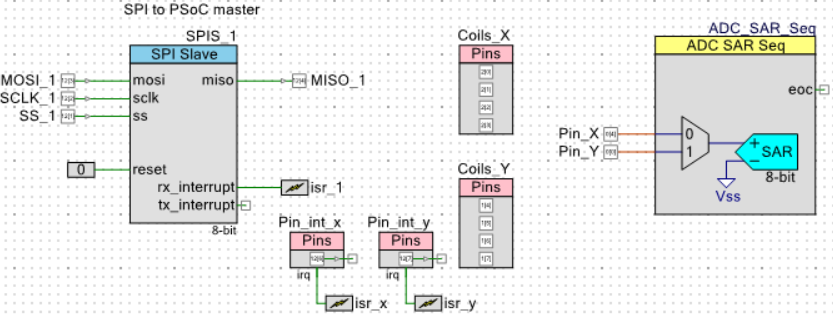
\includegraphics[scale=0.48]{Screenshots/PSoC_TopDesign_X_Y.png}
\caption{PSoC TopDesign for motorstyring og sensoraflæsning}
\label{PSoC_TopDesign_X_Y}
\end{figure}

SPI forbindelsen vil ikke forklares her. Der henvises til afsnit xx for uddybning af denne.

Når der skal detekteres for en flaske tændes ADCen og det analoge signal fra sensoren konverteres til digitale værdier som aflæses. For hvert 10. step (se linje 538 og 559 i main.c), motoren tager, læses en gang fra sensoren. Hvis sensoren detekterer begge kanter på vinflasken vil der på PSoCen ske en kalkulation af hvor midten af flasken er. Herefter vil x- og y-akserne, og dermed åbningsmekanismen, bevæge sig ind på midten af flasken.

\subsubsection{Sensor}
Sensorerne detekterer så længe der er tilkoblet Vcc og GND til dem. I projektet betyder det at sensorerne konstant vil prøve at detektere, men at der i koden kun aflæses fra dem når det er relevant. Dette gøres vha. den sekventielle SAR ADC fra TopDesignet.

\subsubsubsection{Sekventiel SAR ADC} \\
Sequencing SAR ADC komponenten fra Figur \ref{PSoC_TopDesign_X_Y} består af en digital multiplexer, som udgør det sekventielle i ADCen. Yderligere findes en SAR ADC, der konverterer det analoge signal fra sensoren til en digital værdi i PSoCen. Der henvises til bilag xx for datablad for den sekventielle SAR ADC.

Den digitale multiplexer kan tage to input, 0 eller 1. Disse værdier bestemmer hvilken sensor der skal læses fra. Når multiplexeren modtager 0 læses fra x-aksen mens der læses fra y-aksen når den modtager 1. Dette styres fra main.c med funktionen "ADC\_SAR\_Seq\_GetResult16(uint16 chan)", hvor "chan" er den port der læses fra. I main.c er 0 og 1 repræsenteret som "X" og "Y" - defineret i "enum axes" linje 63.

SAR ADC-kredsløbet indeholder en DAC, en komparator og et register til at oversætte det analoge signal fra sensoren til en digital værdi. Outputtet fra ADCen er et antal counts der med funktionen "int32 ADC\_SAR\_Seq\_CountsTo_mVolts(int16 adcCounts)" koverteres til mVolt.

SAR er den måde som ADCen behandler dataene fra sensoren på. Successive approximation register fungerer ved at registret spørger efter en given værdi. Alt efter om den reelle værdi er højere eller lavere er outputtet henholdsvis et binært 1 eller 0. Registret vil spørge indtil en given resolution er opnået og en tilnærmet værdi er opnået.

Nedenstående tabel viser hvordan registret behandler konverteringer. Det er et tænkt scenarie hvor resolutionen er 8 bit.

\begin{table}
\begin{tabular}{| l | c |}
Adspurgt værdi & Binært output\\\hline
128 & 1\\\hline
128 + 64 & 0\\\hline
128 + 32 & 1\\\hline
128 + 32 + 16 & 0\\\hline
128 + 32 + 8 & 1\\\hline
128 + 32 + 8 + 4 & 1\\\hline
128 + 32 + 8 + 4 + 2 & 0\\\hline
128 + 32 + 8 + 4 + 1 & 1\\\hline
Resultat & 10101101\\\hline
\end{tabular}
\end{table}

I tabellen ses det at det endelige resultatet afspejler de enkeltvise delresultater, hvor første delresultat svarer til MSB (most significant bit) og sidste til LSB (least significant bit).

Resolutionen i PSoC designet er sat til 8. Dette er gjort fordi en større nøjagtighed ikke er nødvendig. Sensorens vigtigste egenskab i WinePrep er ikke den målte afstand, men om der sker et skift i aflæst værdi, og dermed, et skift i afstand. Desuden bruges sensoren til at validere flaskens type, og der er afstanden heller ikke nødvendig. Afstanden måles mere præcist i motorernes steps. Se evt. afsnit xx for stepmotorer.

Figur \ref{ADC_SAR_SEQ} viser konfigureringen af ADCen. "Free Running" som sample mode er valgt fordi det er vigtigt at der konstant aflæses fra sensorerne og dermed sammenlignes om der er sket en ændring.

\begin{figure}[H]
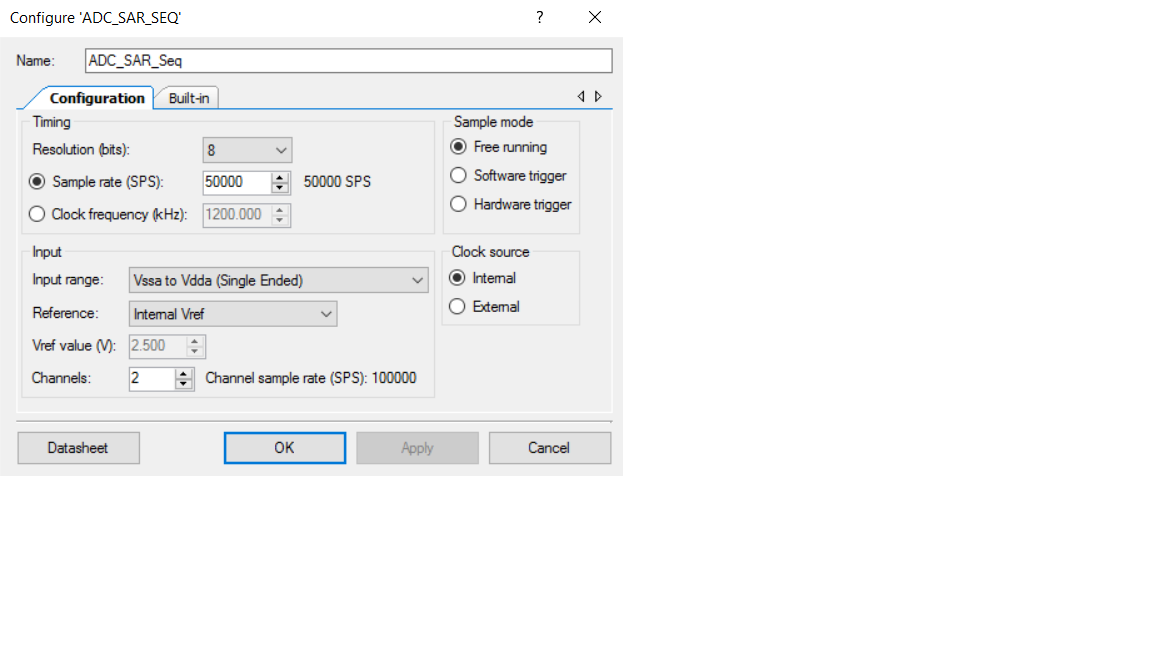
\includegraphics[scale=0.7]{Screenshots/ADC_SAR_SEQ.png}
\caption{Konfigurering af sekventiel SAR ADC}
\label{ADC_SAR_SEQ}
\end{figure}

Som det ses på figur \ref{PSoC_X_Y_pin_configuration} aflæses sensoren på x-aksen på port 0 pin 4 mens detekteringen på y-asken aflæses på port 0 pin 0 på PSoCen. Gennem ADCen fås et decimaltal som svarer til en afstand. Den digitale værdi for afstanden er opgivet i Volt. Sammenhængen mellem Volt og afstand i cm kan ses i databladet for sensoren på figur 4.

\begin{figure}[H]
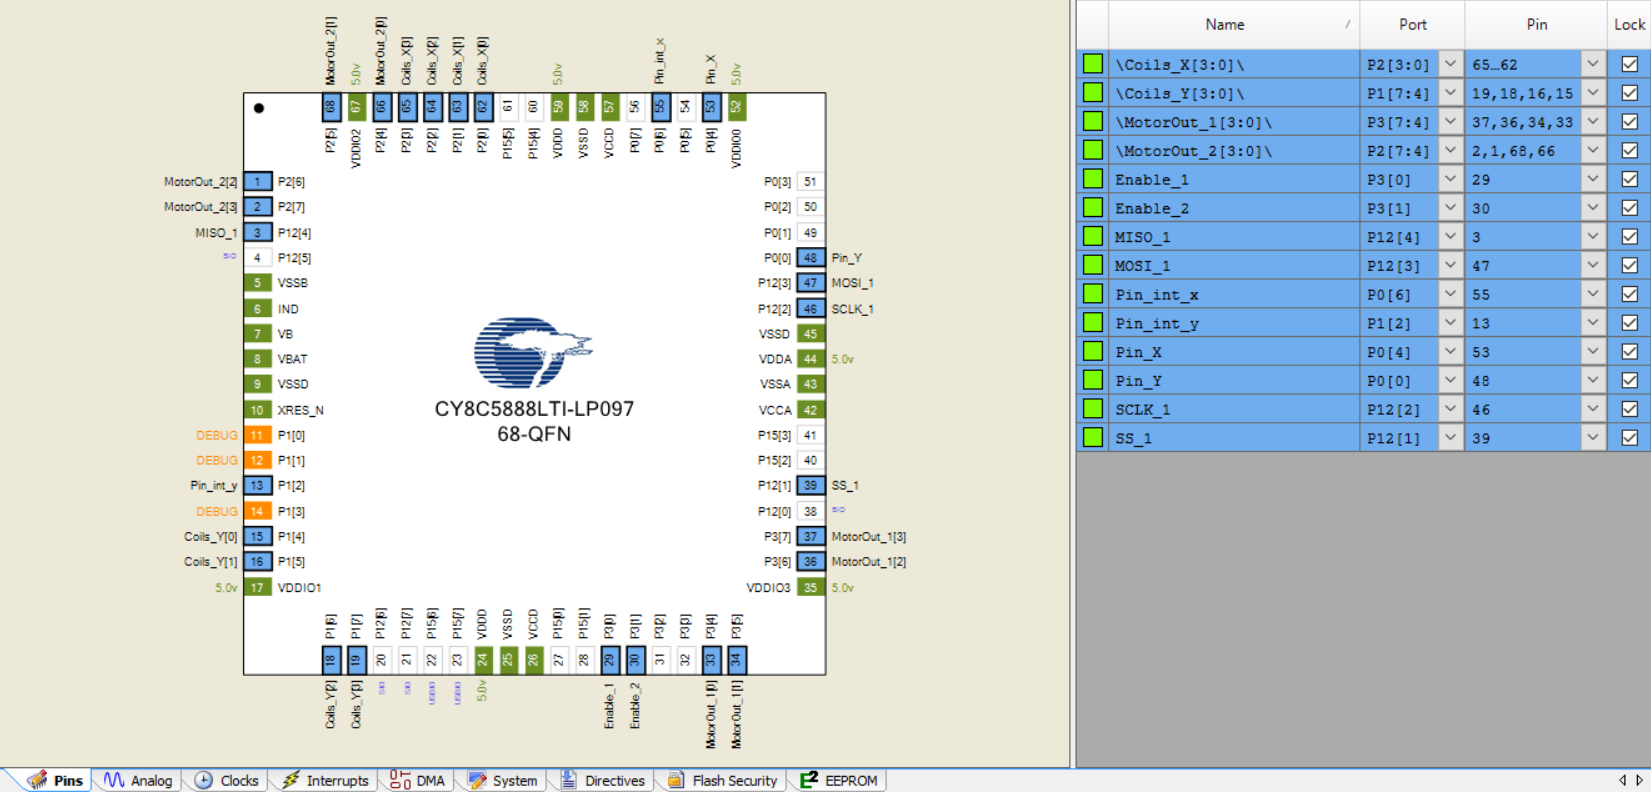
\includegraphics[scale=0.22]{Screenshots/PSoC_X_Y_pin_configuration.png}
\caption{Pin diagram for hele designets komponenter}
\label{PSoC_X_Y_pin_configuration}
\end{figure}

\subsubsection{Motor}
Coils\textunderscore x og Coils\textunderscore y fra figur \ref{PSoC_TopDesign_X_Y} skrives til for at styre stepmotorernes spoler. Linje 3 og 4 i main.c definerer start positionen for motorerne. Hver bit er tilknyttet en bestemt spole. Når denne bit er 1 er spolen tændt, når den er 0 er spolen slukket. Der vil altid være 2 spoler tændt og 2 spoler slukket.

På linje 197 er funktionen rotateRight defineret. Dens opgave er at tænde og slukke spoler således at motoren vil dreje mod højre. Umiddelbart kan det være svært at gennemskue hvad der sker i koden. Nedenstående eksempel udpensler 4 steps. Der tages udganspunkt i x-aksen hvorfor det er xStep fra linje 3 der benyttes. Dennes start position er 0b1100, eller i et helt byte, 0b00001100. Første kolonne fra venstre kolonne er første (venstre) parentes fra linje 199, anden kolonne er anden parentes, tredje kolonne er resultatet af anden parentes multipliceret med 15 og fjerde kolonne er det endelige resultat der returneres fra funktionen.

\begin{table}
\begin{tabular}{| l | c | c | c |}
1. parentes & 2. parentes & 2. parentes \bullet 15 & Resultat\\\hline
0b00000110 & 0b01100000 & 0b00000000 & 0b00000110\\\hline
0b00000011 & 0b00110000 & 0b00000000 & 0b00000011\\\hline
0b10000001 & 0b00011000 & 0b00001000 & 0b00001001\\\hline
0b11000000 & 0b00001100 & 0b00001100 & 0b00001100\\\hline
\end{tabular}
\end{table}

Sidste række i tabellen viser at den er tilbage til udgangspunktet.

Samme forløb gælder for funktionen rotateLeft.

\subsection{ULN2003AN board}
Til at styre motorens fire faser anvendes fire transistorer. I stedet for fire individuelle transistorer er en chip, ULN2003AN, anvendt. Chippen indeholder 7 NPN Darlington transistor par hvor af kun 4 af parrene benyttes til motorstyringen. Værkstedet på studiet har stillet boards til rådighed hvor chippen befinder sig på. Datablad for ULN2003AN kan findes i bilag xx.

På boardet er desuden en socket til at koble motoren direkte på, en kondensator, 4 lysdioder til at indikere hvilken fase der er tændt, 4 formodstande til lysdioderne, en jumper, 2 pins til forsyningsspænding og 4 input pins fra PSoCen.

Boardet kan ses på figur \ref{print_forside}.

\begin{figure}[H]
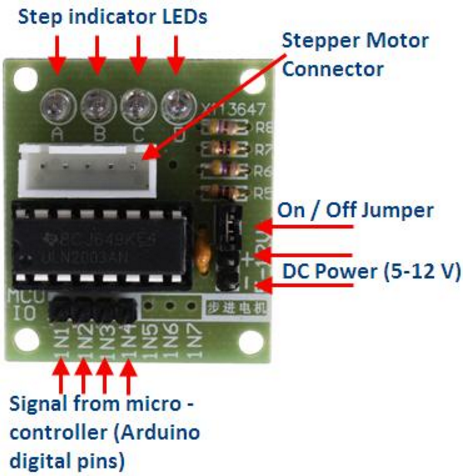
\includegraphics[scale=0.75]{Screenshots/ULN2003AN_board.png}
\caption{Forside af board for styring af unipolær motor}
\label{print_forside}
\end{figure}

\section{Test}
Modultesten blev gennemført ved at benytte UART forbindelse fra en PC til PSoCen. Integrationstesten blev gennemført med SPI forbindelse fra master PSoCen. Opstilling af modultest kan ses på figur \ref{x_sensor_start} som også viser at motor og sensor for x-akse aktive.

\begin{figure}[H]
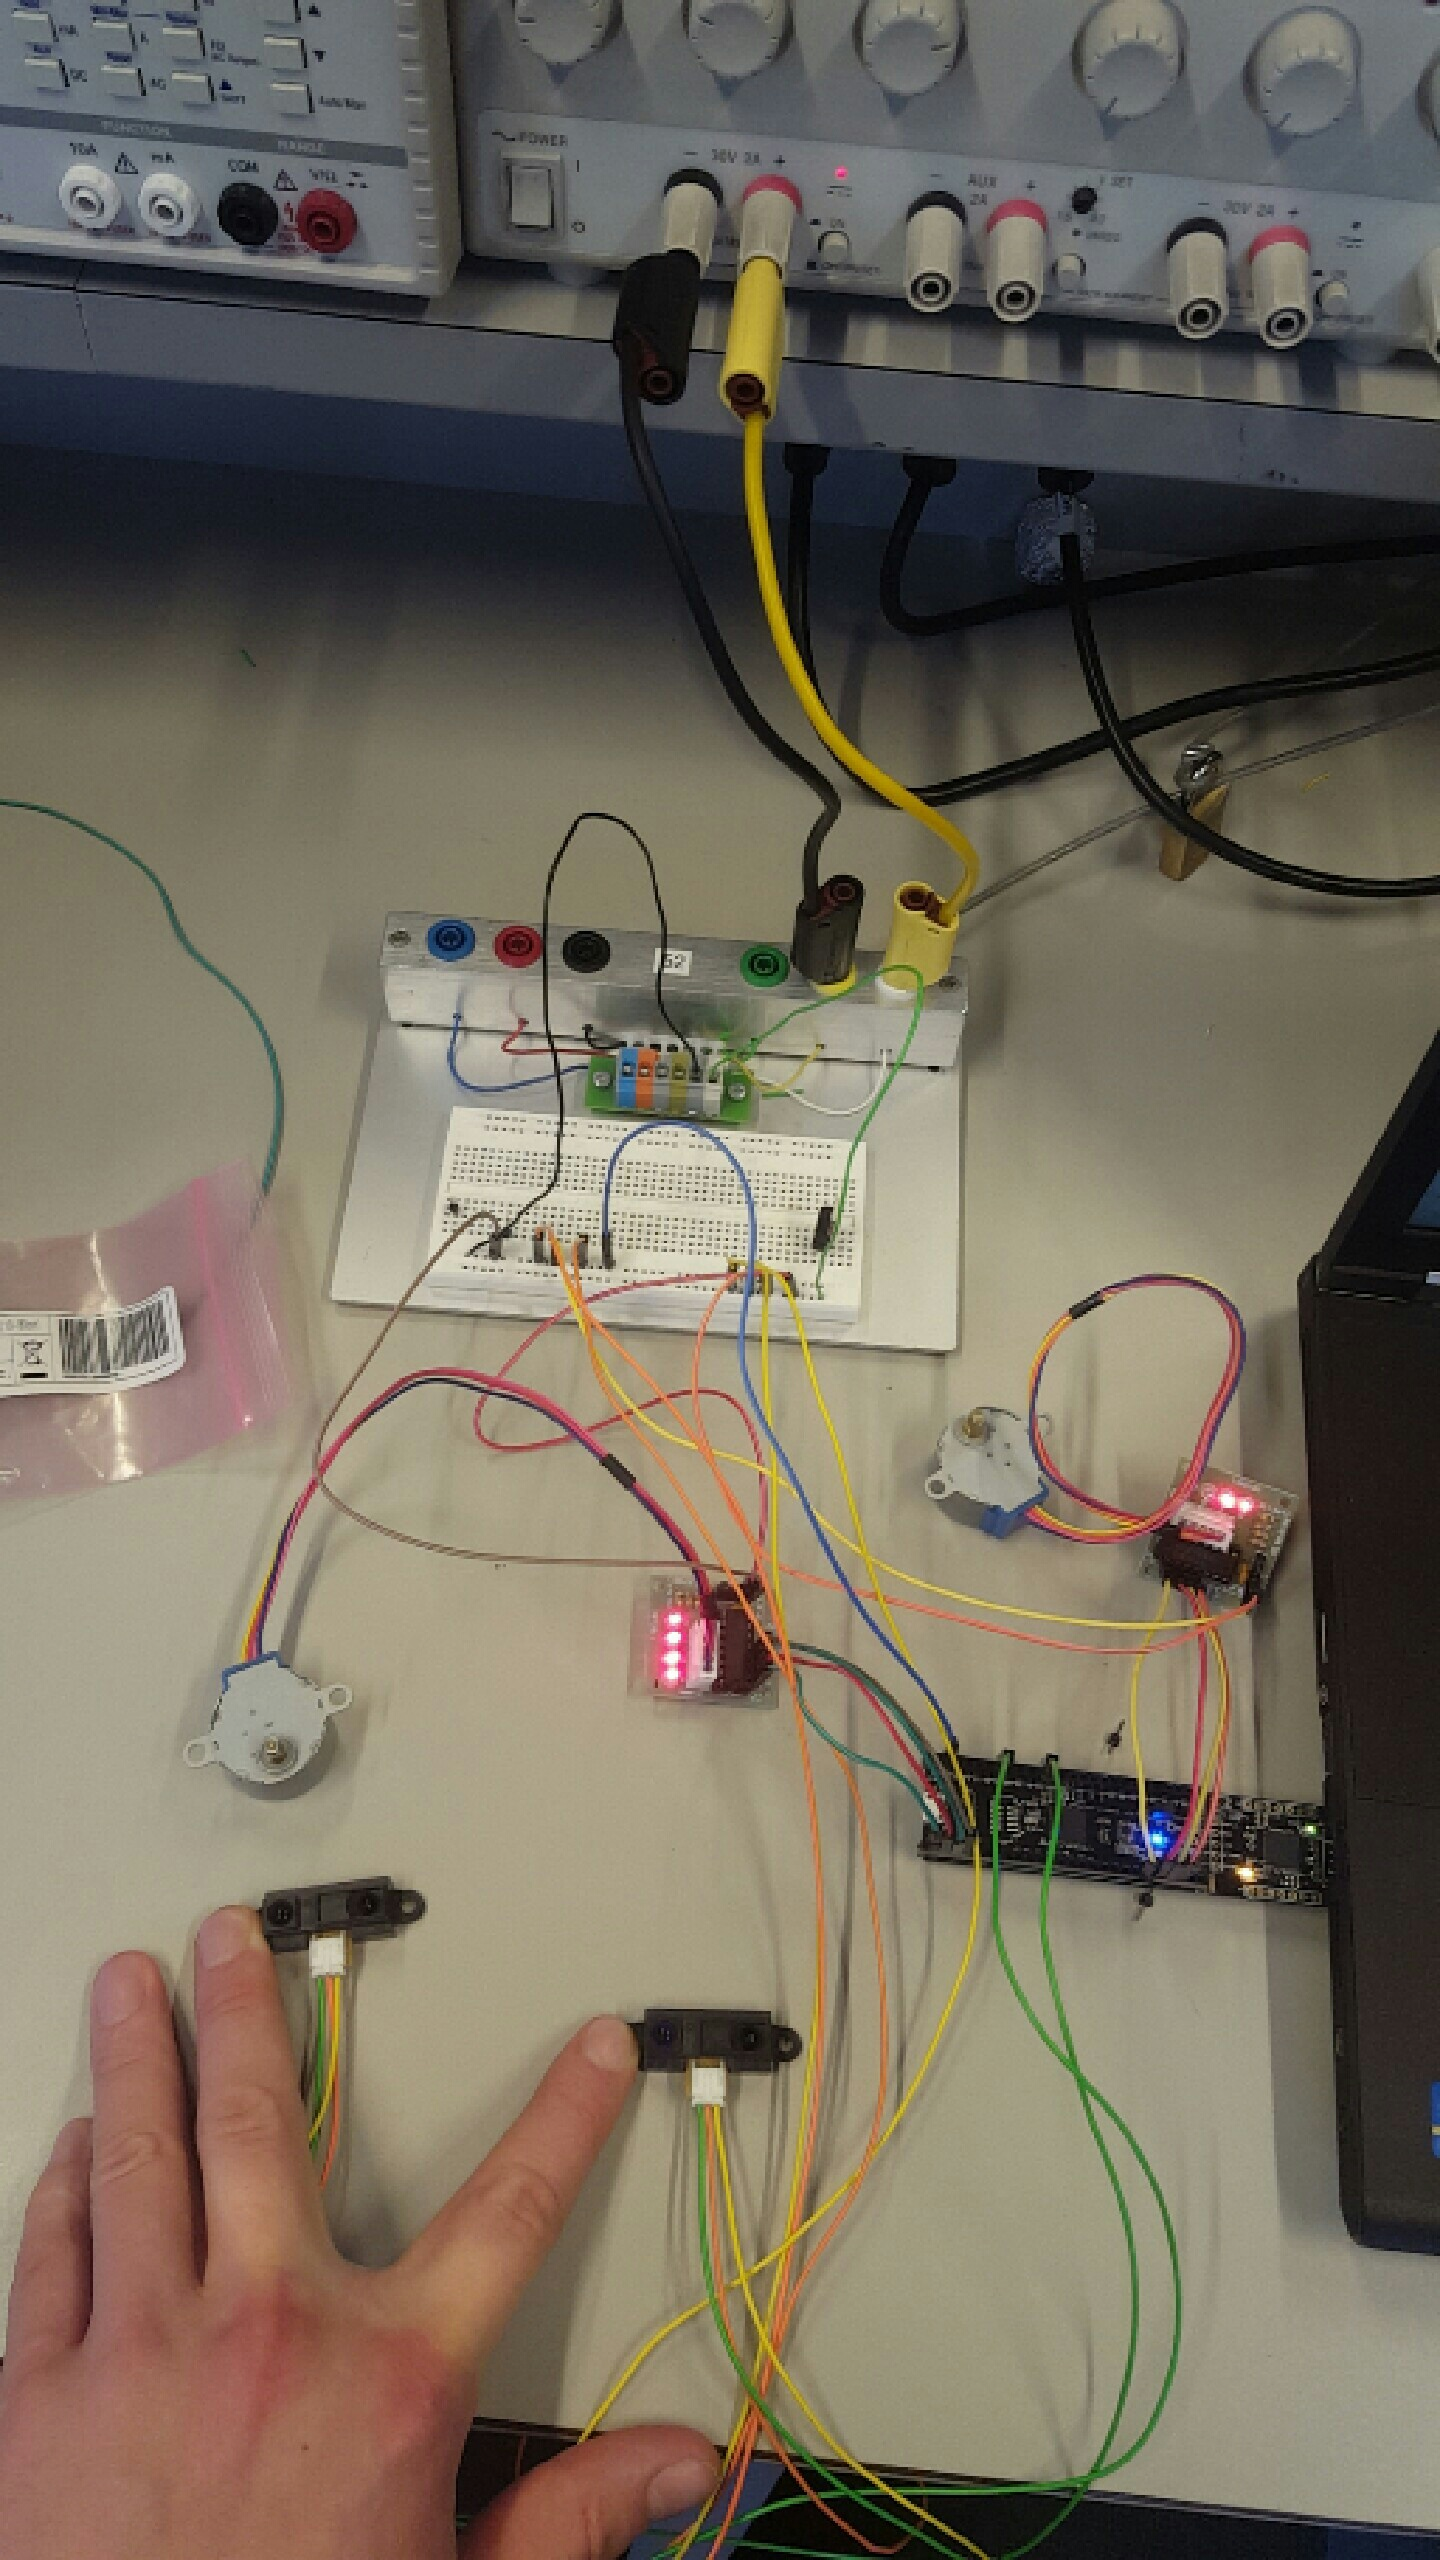
\includegraphics[scale=0.068]{Screenshots/x_sensor_start.jpg}
\caption{Opstilling under modultest}
\label{x_sensor_start}
\end{figure}

Pins er konfigureret fra PSoC til ULN2003AN boardet som vist i opstillingen og på figur \ref{PSoC_X_Y_pin_configuration}. Desuden er PSoCen tilsluttet Vcc og GND fælles med strømforsyning og ULN2003AN boardet. En permanent placeret strømforsyning fra E-LAB er anvendt.

For at sikre at der detekteres indenfor det relevante område, 10-20 cm fra afstandsmåleren, er tests blevet gennemført for at dokumentere hvilke værdier afstanden aflæses i. Sammenhæng mellem afstand og værdier kan ses i nedenstående tabel. Disse værdier er ikke omregnet til Volt, men afstand er målt med tommerstok.
\begin{table}[H]
\begin{tabular}{| l | r |}
	Afstand i cm & Værdi\\\hline
	Uden for rækkevidde & 6\\\hline
	10 & 134\\\hline
	12 & 124\\\hline
	14 & 107\\\hline
	16 & 93\\\hline
	18 & 80\\\hline
	20 & 72\\\hline
	22 & 70\\\hline
	\label{Afstand-vaerdier}
\end{tabular}
\end{table}

Afstandsmåling udenfor rækkevidde er foretaget ved at lade sensoren detektere fra et bord mod loftet af E-LAB, hvilket giver en minimumsafstand på langt over 80 cm, som sensorens rækkevidde er.

Dette kan ikke umiddelbart sammenlignes med figur 4 i databladet for sensoren fordi både værdier og graf ikke er ens. Dog kan disse værdier bruges til at definere minimums- og maksimumsafstande.

I koden er maksimumsafstand defineret som LOW = 72, dvs. hvis værdien fra afstandssensoren aflæses til under denne værdi, ignoreres den. I koden er der ikke taget hensyn til at en genstand kan være mindre end 10 cm fra sensoren. Dette skyldes at sensoren i WinePrep-rammen altid vil være placeret i en minimumsafstand af 10 cm fra objektet.

Først blev x-aksen aktiviteret ved at simulere "LOCATE_XY"-kommandoen fra linje 0x01 i main.c. Dette resulterede i billedet fra figur \ref{x_sensor_start}. En hånd blev anbragt foran sensoren og fjernet igen for at simulere en flaske. Y-aksen blev afsøgt for en flaske med samme procedure som for x-aksen - se figur \ref{y_sensor_start}.

\begin{figure}[H]
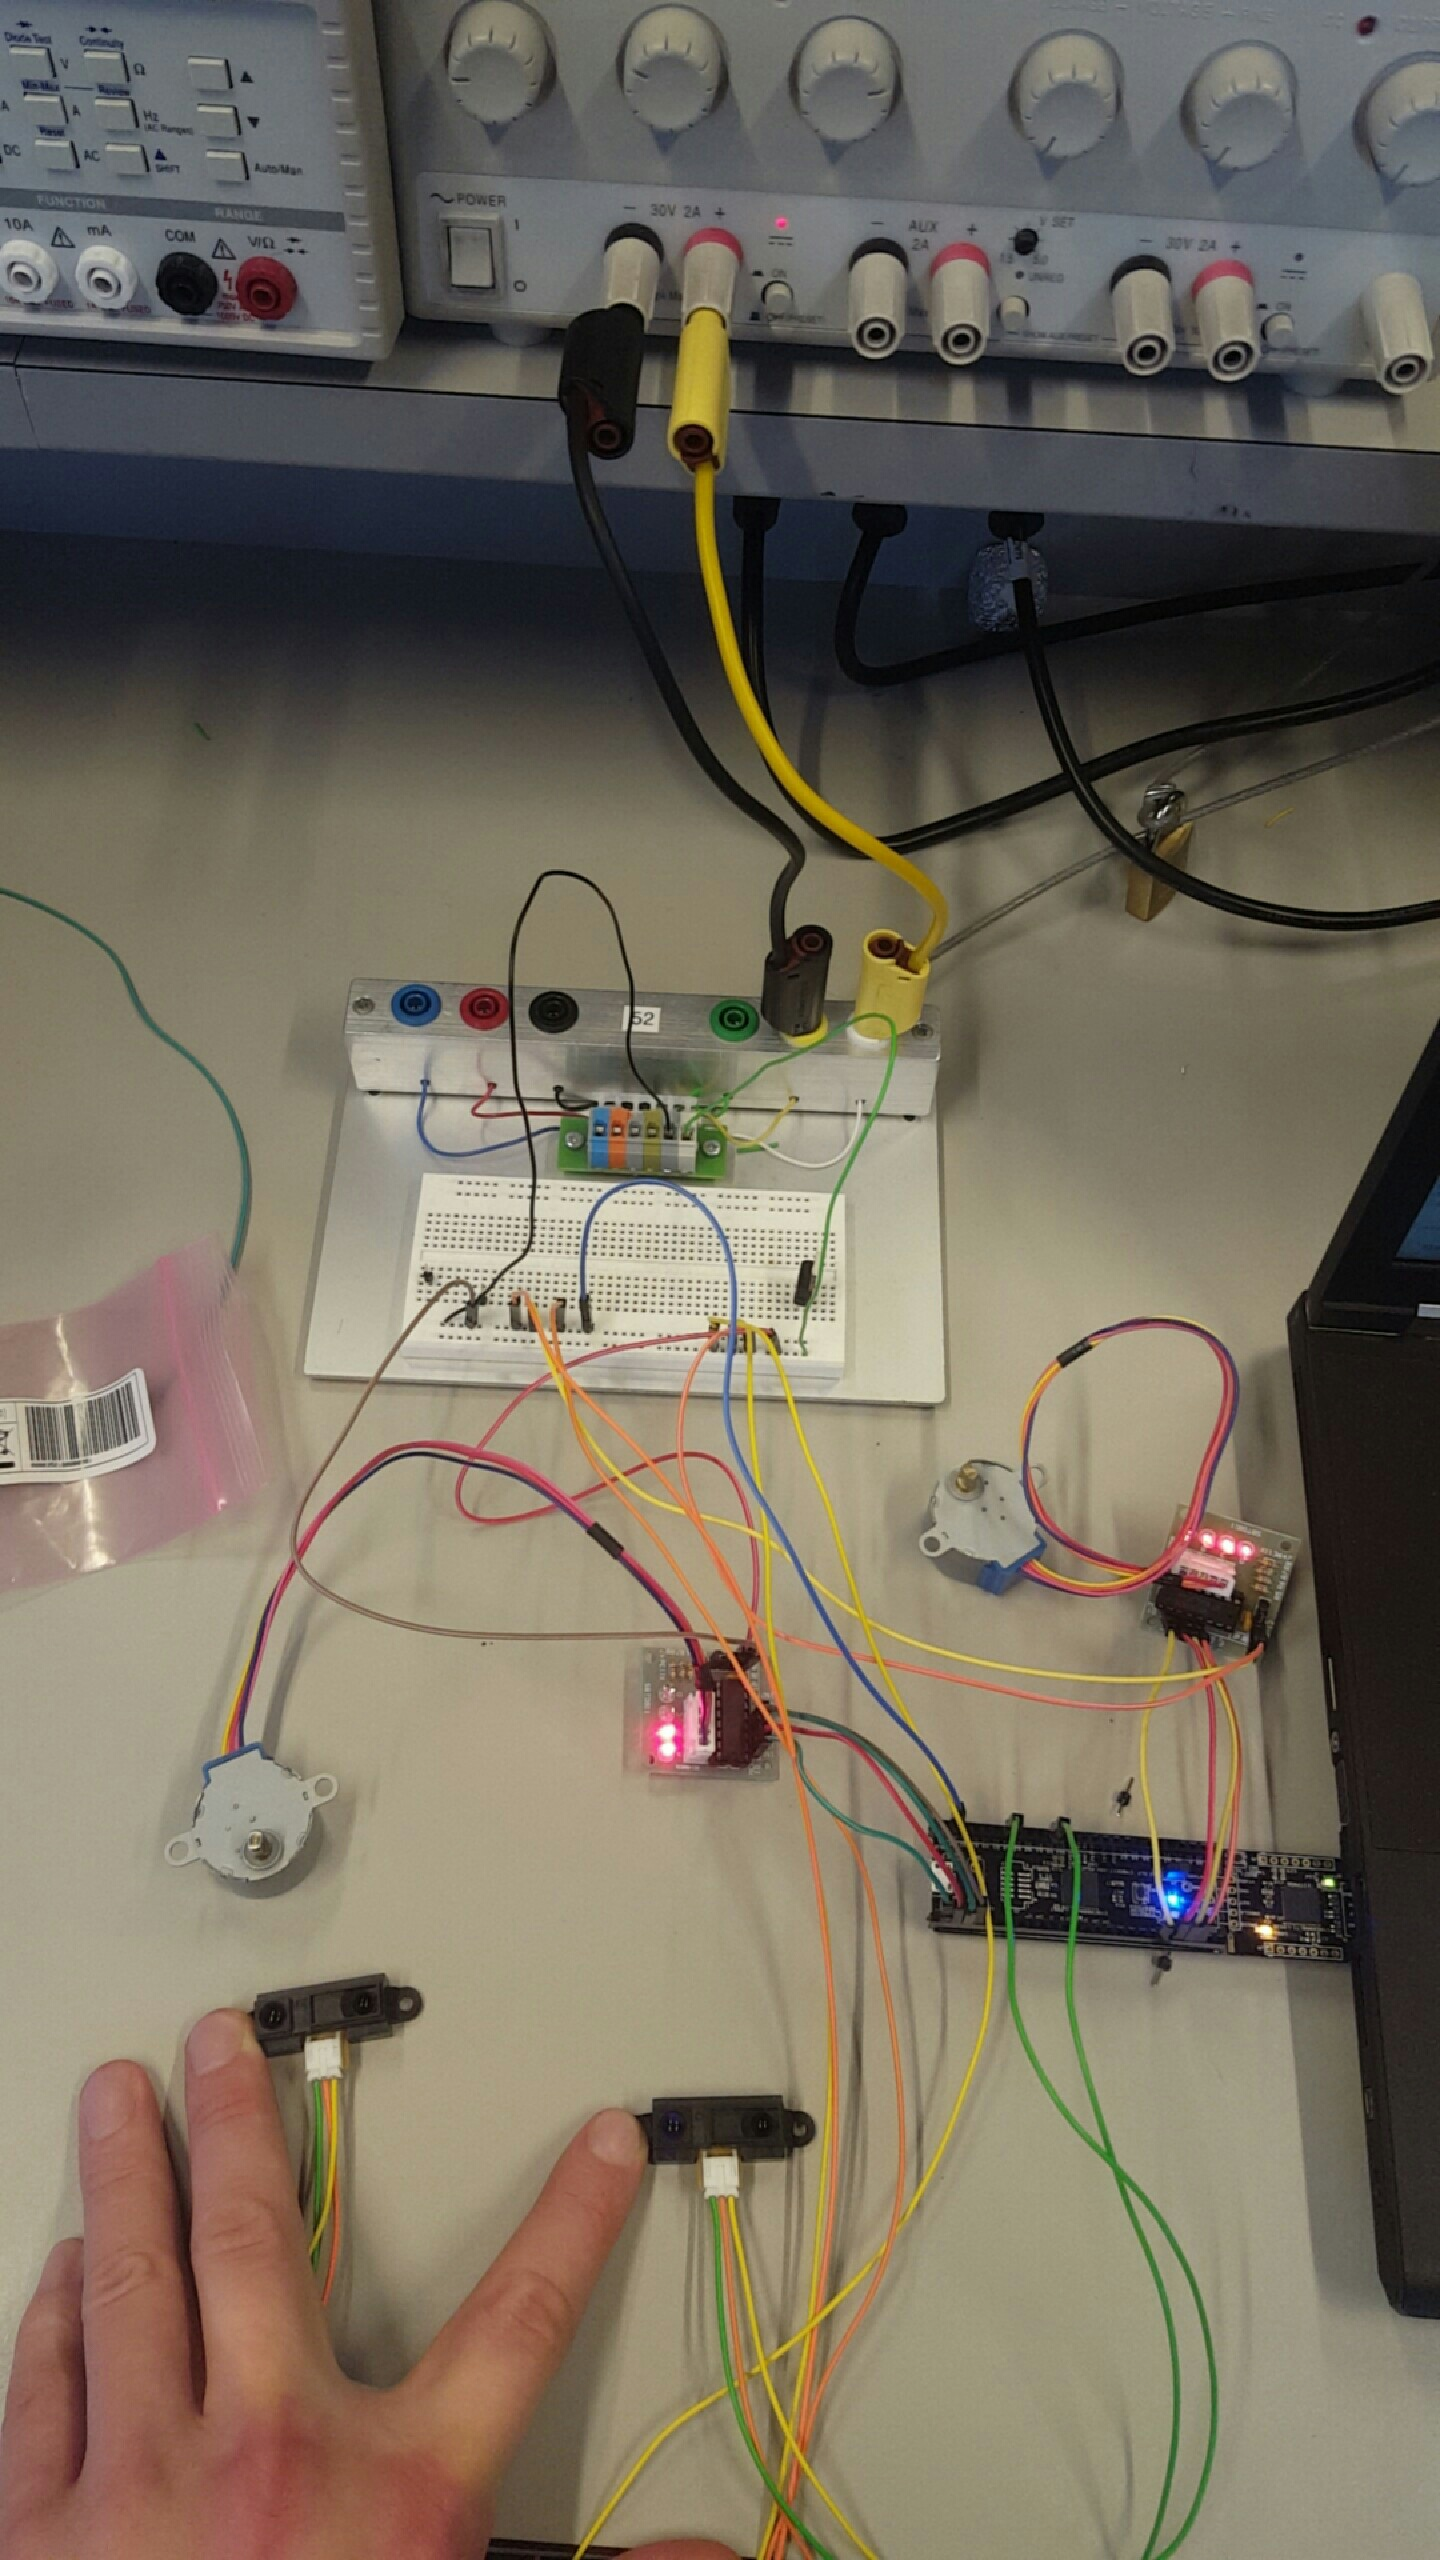
\includegraphics[scale=0.068]{Screenshots/y_sensor_start.jpg}
\caption{Motor og sensor på y-akse aktiveret}
\label{y_sensor_start}
\end{figure}

Figur \ref{End_of_search} viser endt detektering.

\begin{figure}[H]
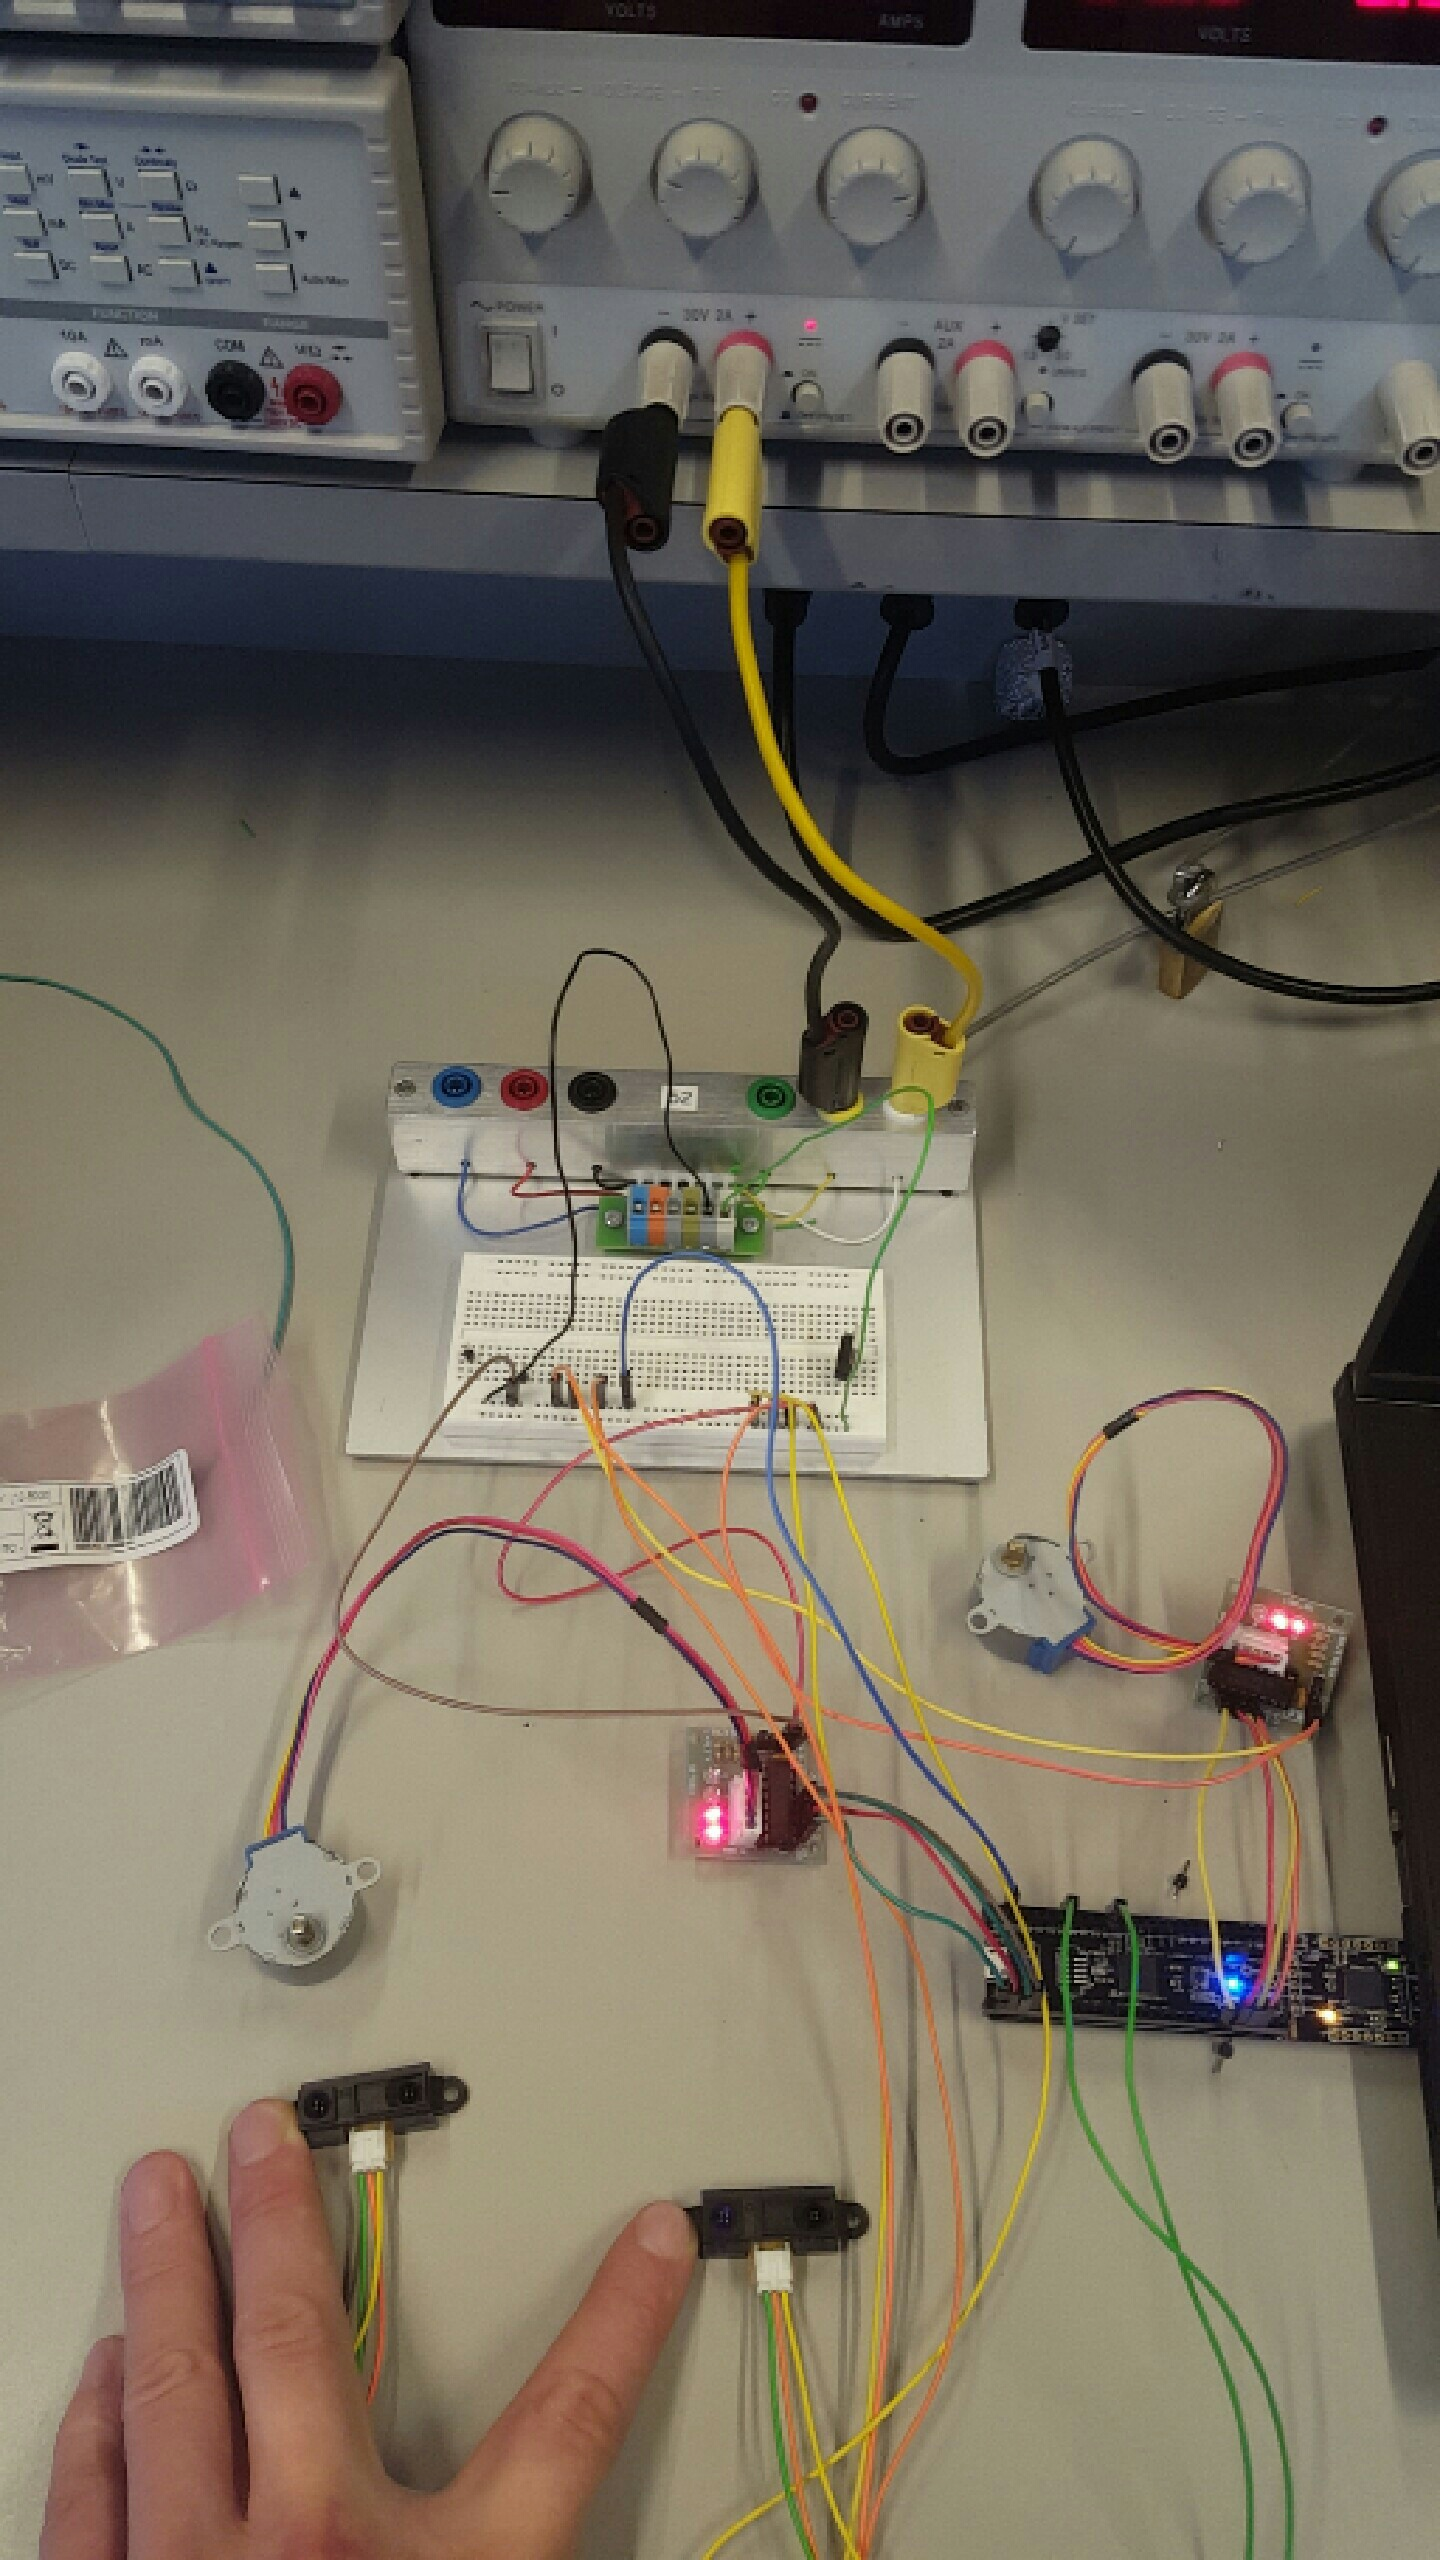
\includegraphics[scale=0.068]{Screenshots/End_of_search.jpg}
\caption{Endt detektering}
\label{End_of_search}
\end{figure}

\section{Resultater}
Følgende figurer viser værdier for målte afstande under testen. Disse kan sammenlignes med tabel \ref{Afstand-vaerdier}. Hovedformålet med denne modultest er at undersøge om der sker en korrekt validering for detektering af en eventuel flaske.

\begin{figure}[H]
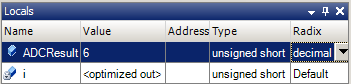
\includegraphics[scale=1]{Screenshots/Sensor-uden-genstand.png}
\caption{Afstandsmåling uden for rækkevidde}
\label{sensor_uden_genstand}
\end{figure}

Denne test er i og for sig underordnet, men er taget med for at dokumentere hvilken værdi en afstandsmåling uden for rækkevidde har. Dette vil kunne bruges til at sammenligne værdier for en reel og en ureel måling.

\begin{figure}[H]
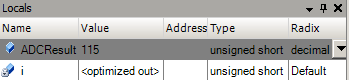
\includegraphics[scale=1]{Screenshots/Sensor-12cm.png}
\caption{Afstandsmåling ved 12 cm}
\label{Sensor_12cm}
\end{figure}

\begin{figure}[H]
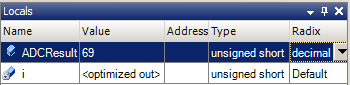
\includegraphics[scale=1]{Screenshots/Sensor-22cm.png}
\caption{Afstandsmåling ved 22cm}
\label{Sensor_22cm}
\end{figure}

Ved testen sås det at afstandsmåling ved 22 cm resulterede i en uendelig loop i koden. Ved en afstandsmåling ved 12 cm sås det ønskede resultat, nemlig, at motoren bevægede sig indtil den aflæste værdi var mindre end LOW. Dette resulterede i at motoren roterede i modsat retning indtil en simuleret midte af flasken var nået. 

For at se testen på video refereres til bilag xx.

\section{Diskussion}
Testen betragtes generelt som godkendt, dog ville en test med flere afstandsmålinger give et bedre billede. For at sikre den bedst mulige test skulle der have været testet ved grænserne, 10 og 20 cm. Dog betragtes denne test som gennemført af den årsag at den afviste en afstand som lå over den øvre grænse. Samtidig blev en test indenfor det godkendte interval, 10-20 cm, gennemført.